


                           
% Overleaf: XeLaTeX
\documentclass[UTF8,12pt,a4paper,openany]{ctexbook}

\usepackage{amsmath,amssymb}
\usepackage{booktabs,tabularx,array}
\usepackage{graphicx,float}
\usepackage{xcolor}
\usepackage{tikz}
\usetikzlibrary{arrows.meta,positioning,fit,calc}
\usepackage[margin=2.6cm]{geometry}
\usepackage{hyperref}
\hypersetup{hidelinks}

% 图片占位命令：
% #1：预留高度；#2：框内说明；#3：图题；#4：引用标签
% 后续可将整个 \placeholderfigure 命令替换为正式插图代码。
\newcommand{\placeholderfigure}[4]{%
    \begin{figure}[htbp]
        \centering
        \fbox{%
            \parbox[c][#1][c]{0.85\linewidth}{%
                \centering
                \color{black}#2
            }%
        }
        \caption{#3}
        \label{#4}
    \end{figure}
}

\begin{document}

\tableofcontents

\chapter{移动机器人硬件与软件系统设计}
\label{chap:system}

\section{机器人整体结构}

本文以四轮独立转向驱动底盘为移动平台，采用Jetson Orin NX作为上位计算单元，并配置激光雷达及RGB-D相机，构建面向温室棚架环境的移动机器人系统。四个车轮均具有独立转向和驱动能力，可实现纵向、横向及旋转运动。为提高电机通信的实时性及故障状态下的独立保护能力，系统拟增设STM32底层控制器；该控制板尚处于选型与接口设计阶段。整机结构如图\ref{fig:robot-photo}所示。

\placeholderfigure{5cm}{整机实物图（待补充）}{移动机器人整机结构}{fig:robot-photo}

目标系统采用上位计算与下位执行分工的控制架构。Jetson负责Web交互、环境感知、定位建图、路径规划和四轮运动学解算；拟增加的STM32负责接收轮级目标、调度两路CAN、采集电机反馈及执行通信超时保护。现阶段原型系统由Jetson通过SocketCAN直接连接两路执行器总线，用于验证电机协议、轮序映射和上层控制算法；后续在不改变ROS~2上层接口的前提下，将硬件通信部分替换为Jetson--STM32通信接口。目标硬件连接关系如图\ref{fig:system_architecture}所示。

\begin{figure}[htbp]
    \centering
    \IfFileExists{硬件结构.pdf}{%
      \includegraphics[width=0.95\textwidth]{硬件结构.pdf}%
    }{\fbox{\parbox[c][4cm][c]{0.85\linewidth}{\centering 硬件结构图（待上传）}}}
    \caption{移动机器人硬件系统架构}
    \label{fig:system_architecture}
\end{figure}

\section{四轮独立转向驱动底盘}

底盘采用四轮独立转向、四轮独立驱动结构。转向执行器为达妙DM4340P电机，行走系统由四个中菱轮毂电机及两台ZLAC8015D驱动器组成。转向电机采用位置--速度控制，行走驱动器采用CANopen速度控制。目标方案中，各轮转角与轮速由Jetson统一计算，再发送至STM32，由STM32分别通过转向CAN总线和行走CAN总线下发。现阶段在STM32控制板完成前，Jetson侧驱动直接访问两路SocketCAN接口，以支持软件和电机通信链路的先期验证。

底盘实际安装尺寸存在非对称性，且转向机构受到允许角度范围约束。后续运动学建模采用各车轮实际位置，结合驱动轮正反转处理有限转角下的运动需求。

\section{控制与感知硬件}

底盘底层控制器拟选用具有不少于两路独立CAN接口、硬件定时器及看门狗资源的STM32器件，STM32G4系列可作为候选，最终型号以接口数量、封装引脚、存储资源和控制板设计结果为准。一路CAN用于连接DM转向电机，另一路CAN用于连接ZLAC8015D行走驱动器。Jetson与STM32之间拟采用USB虚拟串口、USB自定义通信或独立CAN链路中的一种；具体物理接口将在控制板选型后通过通信时延与抗干扰试验确定，本文不预先将其限定为已经实现的USB-CAN连接。

STM32端计划完成轮级目标解析、序号及校验检查、周期报文调度、电机反馈聚合、指令超时停车和故障状态上传。升降台继电器控制可在接口资源允许时并入底盘STM32；SCARA机械臂仍采用独立控制器，使底盘和机械臂的实时执行任务相互隔离。照明、状态指示及电源检测接口按实际需要配置。实体急停采用独立于Jetson、Web页面和STM32软件逻辑的硬件安全链路。

Jetson Orin NX运行ROS 2系统，通过USB连接激光雷达与Intel RealSense D435i相机，分别获取平面扫描和RGB-D数据。传感器标定、坐标变换及融合方法在环境感知章节介绍。

\section{机器人软件系统架构}

软件系统按照任务交互、感知定位、规划决策、运动控制及底层执行组织。Jetson端负责人工操作与自主导航指令仲裁、地图构建、局部规划、四轮逆运动学及转向协调；目标架构中的底盘STM32负责电机通信、反馈采集和底层安全执行，机械臂控制器负责SCARA执行控制。车体速度指令由Jetson转换为四轮转角与轮速目标，经上位机--下位机协议发送至STM32，再由STM32通过两路CAN发送至执行器；电机状态沿相反方向聚合反馈。STM32尚未接入时，Jetson侧硬件接口临时承担CAN协议转换与状态采集，以保持上层话题和控制器接口不变。

环境感知采用RTAB-Map进行定位建图，并利用Nvblox维护局部三维环境信息；棚架结构识别及语义编号为后续研究内容。导航模块采用Nav2框架，有限转向角约束下的规划器设计在后续章节展开。各功能模块的实现状态以实验验证结果为准。


\section{研究目标与拟创新点}

本研究围绕两个问题展开：一是有限转向角造成的四轮轮向切换和轨迹执行不连续；二是多层棚架环境中三维几何地图缺少明确的对象身份及层级关系。拟开展以下研究：

（1）在非对称四轮运动学基础上分析转向角限制和速度空间边界，研究有限转向角下的轮向切换规律，并探索将相关约束引入局部规划器的方法。

（2）结合RGB-D视觉、RTAB-Map定位及Nvblox局部三维重建，提取棚架几何特征，利用多帧关联建立包含棚架编号、层级、边界和朝向的结构化语义地图。

以上内容为拟开展的研究工作。算法差异及性能改进需在后续实验中验证，不预先作为已完成创新成果。

\section{本章小结}

本章介绍了机器人硬件组成、通信连接及软件功能划分，为后续四轮运动学建模、环境感知与局部运动规划提供系统基础。

% 本文件作为独立章节插入主文档，建议放在“移动机器人硬件与软件系统设计”之后、
% “四轮独立转向驱动底盘运动学建模与控制”之前。
% 本章依据 mobile_base_web_console、mobile_base_swerve_controller 与
% mobile_base_driver 的当前实现撰写；实验数据未完成处保留待测说明。

\chapter{基于Web的机器人监控与遥操作系统设计与实现}
\label{chap:web-control}

为降低移动机器人现场调试和多模块联调的操作复杂度，本文设计并实现了一套基于Web的
机器人监控与遥操作系统。该系统运行于机器人上位计算机，局域网内的操作人员无需安装
专用客户端，仅通过浏览器即可完成系统状态查看、整车运动控制、工作模式切换、单轮维护、
转向零位标定、地图与三维环境查看以及导航目标下发等操作。

Web系统并不直接计算四轮转角和轮速，而是向ROS~2控制链发布车体速度指令
$[v_x,v_y,\omega_z]^{\mathrm T}$。四轮运动学解算、有限转角下的等效轮向选择、轮速限幅
及对齐联锁由Jetson端底盘控制器完成，相关方法将在第\ref{chap:kinematics-control}章中介绍。
拟增加的STM32只接收轮级目标，负责确定周期的CAN通信、反馈采集和底层故障保护，不重复
执行车体逆运动学。由于STM32控制板尚未完成，现阶段原型系统由Jetson通过SocketCAN直接
连接执行器；后续将保持Web和ROS~2接口不变，仅替换底层硬件通信通路。

\section{系统需求与总体设计}

\subsection{功能需求}

结合机器人装配、标定、遥操作和自主导航实验的实际需要，Web系统的功能需求可归纳为
以下五个方面。

\begin{enumerate}
    \item \textbf{状态监测：}显示控制器、CAN接口、四轮关节、里程计及系统诊断状态，
          使操作者能够判断控制链是否具备运行条件；
    \item \textbf{整车遥操作：}将虚拟摇杆、旋转滑条和典型动作按钮转换为车体三自由度
          速度指令，并支持立即停车；
    \item \textbf{维护与标定：}在独立维护模式下对单个轮组进行低速转向和行走测试，
          读取转向电机绝对位置并保存机械零位；
    \item \textbf{环境信息显示：}显示RTAB-Map二维占据栅格、机器人轨迹、RGB-D图像、
          Nvblox三维网格以及棚架语义对象；
    \item \textbf{导航交互：}在地图中选取目标位置和目标朝向，通过Nav2动作接口提交或
          取消导航任务。
\end{enumerate}

除上述功能需求外，系统还需满足控制模式互斥、输入限幅、通信中断停车及配置修改受限等
安全要求。需要说明的是，浏览器中的停车按钮、软件看门狗和通信超时均属于软件保护，
不能替代能够切断驱动动力的实体急停装置。

\subsection{系统总体架构}

系统采用浏览器、Web服务与ROS~2接口、Jetson运动控制、STM32实时执行和电机驱动的分层
结构，如图\ref{fig:web-architecture}所示。浏览器端由HTML、CSS和JavaScript实现，负责
产生操作指令并绘制状态信息；Web服务端由Python实现，在同一进程中运行HTTP服务器和
ROS~2节点，完成HTTP/JSON数据与ROS~2消息、服务及动作之间的转换；Jetson端底盘控制器
负责运动学解算和轮级约束处理；拟开发的STM32执行层负责上位机通信、双CAN报文调度、
反馈聚合和超时保护。图中虚线部分为尚待硬件实现的目标链路。

\begin{figure}[htbp]
    \centering
    \begin{tikzpicture}[
        node distance=8mm and 11mm,
        block/.style={draw,rounded corners,align=center,minimum height=10mm,
                      text width=3.25cm,font=\small},
        line/.style={-Latex,thick}
    ]
        \node[block] (browser) {浏览器前端\\状态显示与操作输入};
        \node[block,right=of browser] (web) {Web服务与ROS~2节点\\HTTP/JSON接口与状态聚合};
        \node[block,right=of web] (controller) {Jetson运动控制器\\运动学解算与约束处理};
        \node[block,below=of controller,dashed] (stm) {拟开发STM32执行层\\双CAN调度与安全保护};
        \node[block,left=of stm] (motor) {执行器\\ZLAC行走驱动器与DM转向电机};
        \node[block,below=of web] (perception) {感知与导航模块\\RTAB-Map、Nvblox、Nav2};

        \draw[line] (browser)--node[above,font=\scriptsize]{HTTP/JSON} (web);
        \draw[line] (web)--node[above,font=\scriptsize]{\texttt{Twist}} (controller);
        \draw[line,dashed] (controller)--node[right,font=\scriptsize]{轮级目标帧} (stm);
        \draw[line,dashed] (stm)--node[above,font=\scriptsize]{两路CAN} (motor);
        \draw[line,dashed] (motor) to[bend left=18] node[below,font=\scriptsize]{位置/速度反馈} (stm);
        \draw[line,dashed] (stm) to[bend left=18] node[right,font=\scriptsize]{聚合反馈} (controller);
        \draw[line] (controller) to[bend right=25] node[above,font=\scriptsize]{关节与里程计状态} (web);
        \draw[line] (perception)--node[right,font=\scriptsize]{地图、图像、语义对象} (web);
        \draw[line] (web) to[bend left=12] node[left,font=\scriptsize]{导航目标} (perception);
    \end{tikzpicture}
    \caption{基于Web的机器人监控与遥操作系统架构}
    \label{fig:web-architecture}
\end{figure}

当前Web服务节点发布\texttt{/swerve\_controller/cmd\_vel}，四轮四转控制器将车体速度
转换为四个转向位置目标和四个驱动速度目标。目标方案中，Jetson硬件接口将八个轮级目标、
工作模式、命令序号和校验信息封装后发送至STM32；STM32再分别通过行走CAN和转向CAN控制
ZLAC8015D驱动器与DM转向电机。因此，最终网页控制链路可表示为
\begin{equation}
\text{浏览器}
\rightarrow \text{HTTP接口}
\rightarrow \text{ROS~2速度指令}
\rightarrow \text{四轮运动学控制器}
\rightarrow \text{Jetson--STM32接口}
\rightarrow \text{STM32双CAN调度}
\rightarrow \text{执行器}.
\label{eq:web-command-chain}
\end{equation}

状态反馈沿相反方向传输：STM32计划聚合各执行器位置、速度、在线状态和故障码，并携带
反馈序号及时间信息返回Jetson；Jetson硬件接口将其转换为ROS~2关节状态，控制器再根据
轮速反馈计算里程计。Web节点订阅相关话题并转换为浏览器可处理的JSON数据，使操作者能够
同时观察控制输入、车轮实际状态和机器人位姿变化。STM32接入前，上述CAN收发和反馈转换
由Jetson侧SocketCAN驱动完成，作为上层功能验证的过渡实现。

\section{前后端通信与ROS~2数据交互}

\subsection{Web服务实现}

Web服务端采用多线程HTTP服务器处理局域网请求，并在主线程中运行ROS~2节点。两类线程
通过互斥锁保护共享状态，避免HTTP请求与ROS回调同时访问关节、里程计、地图或模式变量时
产生数据竞争。浏览器与服务端之间采用HTTP请求和JSON数据交换，静态页面与控制接口由
同一服务端口提供，默认监听端口为8080。

主要接口如表\ref{tab:web-api}所示。读取类接口用于状态刷新和可视化，写入类接口用于
控制、模式切换、参数修改及标定。服务端对请求字段进行类型、有限值和取值范围检查，
并使用不同HTTP状态码区分参数错误、状态冲突和服务内部错误。

\begin{table}[htbp]
    \centering
    \caption{Web系统主要HTTP接口}
    \label{tab:web-api}
    \begin{tabularx}{\textwidth}{p{1.4cm}p{5.1cm}X}
        \toprule
        方法 & 接口 & 功能 \\
        \midrule
        GET & \texttt{/api/status} & 获取控制模式、控制器、CAN、关节、里程计、诊断及导航状态 \\
        GET & \texttt{/api/map} & 获取二维占据栅格地图及地图元数据 \\
        GET & \texttt{/api/scene3d} & 获取降采样后的Nvblox三维环境数据 \\
        GET & \texttt{/api/racks} & 获取棚架及各层稳定编号、边界和观测状态 \\
        GET & \texttt{/api/config}、\texttt{/api/chassis} & 获取网页限速和底盘硬件配置 \\
        POST & \texttt{/api/control/cmd\_vel} & 下发整车纵向、横向和偏航速度 \\
        POST & \texttt{/api/control/stop} & 取消导航并向运动控制链发送零速度 \\
        POST & \texttt{/api/mode} & 切换禁止、维护或正常控制模式 \\
        POST & \texttt{/api/maintenance/command} & 下发单轮维护转角与转速命令 \\
        POST & \texttt{/api/navigation/goal} & 向Nav2发送目标位姿 \\
        POST & \texttt{/api/navigation/cancel} & 取消当前导航任务 \\
        POST & \texttt{/api/calibration/read}、\texttt{/api/calibration/save} & 读取绝对位置并确认保存转向零偏 \\
        PUT & \texttt{/api/config}、\texttt{/api/chassis} & 更新速度限制或底盘配置 \\
        \bottomrule
    \end{tabularx}
\end{table}

为限制非授权访问，系统可通过环境变量设置访问令牌。启用令牌后，写入类请求需要在
HTTP头中携带认证信息。该措施用于减少局域网内的误操作风险，但当前系统未按公网服务的
威胁模型设计，因此实际部署时仅允许可信局域网访问，不应直接暴露到互联网。

\subsection{状态数据聚合与刷新}

Web节点订阅的主要ROS~2数据及其页面用途如表\ref{tab:web-ros-topics}所示。不同数据源的
产生频率和数据量差异较大，前端采用分级轮询方式：系统状态约每0.5~s刷新一次，摄像机
画面约每1~s刷新一次，三维场景和棚架模型约每1.5~s刷新一次，二维地图约每2~s刷新一次。
这种设计避免将大体量地图或三维数据与高频控制请求绑定在同一刷新周期内。

\begin{table}[htbp]
    \centering
    \caption{Web节点连接的主要ROS~2数据}
    \label{tab:web-ros-topics}
    \begin{tabularx}{\textwidth}{p{5.1cm}p{4.0cm}X}
        \toprule
        话题或接口 & 数据类型 & 页面用途 \\
        \midrule
        \texttt{/joint\_states} & \texttt{sensor\_msgs/JointState} & 四轮转角、轮速及反馈在线状态 \\
        \texttt{/swerve\_controller/odom} & \texttt{nav\_msgs/Odometry} & 机器人位姿、速度和轨迹显示 \\
        \texttt{/rtabmap/map} & \texttt{nav\_msgs/OccupancyGrid} & 二维SLAM地图显示与目标点选择 \\
        \texttt{/rtabmap/localization\_pose} & 定位位姿 & 地图坐标系中的机器人姿态 \\
        \texttt{/nvblox\_node/mesh} & \texttt{nvblox\_msgs/Mesh} & 三维环境点视图 \\
        \texttt{/rack\_map/model} & JSON字符串 & 棚架编号、层级、边界和遮挡状态 \\
        RGB图像与分割调试图像 & \texttt{sensor\_msgs/Image} & 实时图像与目标分割结果 \\
        \texttt{/navigate\_to\_pose} & Nav2动作接口 & 导航目标提交、反馈与取消 \\
        \bottomrule
    \end{tabularx}
\end{table}

二维占据栅格在服务端采用游程编码压缩，并附加版本号。当前端已经持有相同版本时，
服务端仅返回“数据未变化”标志，从而减少重复传输。Nvblox网格在服务端保存增量网格块，
并降采样为适合浏览器绘制的彩色三维点集。棚架对象在显示前根据TF关系转换至地图或
三维场景坐标系；当坐标变换不可用时，系统只显示对象编号列表，而不在不一致坐标系中
强行叠加其几何位置。

\subsection{Jetson与STM32通信接口设计}

为将现有Jetson直连CAN方案迁移至上下位机分层结构，拟在ROS~2硬件接口与STM32之间定义
独立的二进制通信协议。物理层可根据控制板资源在USB虚拟串口、USB自定义通信和独立CAN
链路中选择，但上层数据语义保持一致。相比直接传输编译器内存结构，显式定义帧头、长度、
协议版本、消息类型和字节序可降低上下位机软件升级造成的不兼容风险。

Jetson向STM32发送的轮级目标帧至少包含表\ref{tab:web-command-frame}所列字段。

\begin{table}[htbp]
    \centering
    \caption{拟设计的Jetson至STM32轮级目标帧}
    \label{tab:web-command-frame}
    \begin{tabularx}{\textwidth}{p{3.2cm}p{3.0cm}X}
        \toprule
        字段 & 建议数据类型 & 作用 \\
        \midrule
        帧头与协议版本 & 无符号整数 & 帧同步及上下位机版本兼容检查 \\
        消息类型与载荷长度 & 无符号整数 & 区分控制、配置、心跳和复位等消息 \\
        命令序号 & 递增无符号整数 & 识别重复、乱序和长时间未更新的命令 \\
        工作模式与使能位 & 枚举及位字段 & 明确禁止、正常或维护状态 \\
        四轮转向目标 & $4\times\mathrm{float32}$ & 四个车轮的目标转角，单位为rad \\
        四轮驱动目标 & $4\times\mathrm{float32}$ & 四个车轮的目标角速度，单位为rad/s \\
        上位机时间信息 & 无符号整数 & 用于时效判断和通信性能测量 \\
        CRC校验 & 无符号整数 & 检测传输错误 \\
        \bottomrule
    \end{tabularx}
\end{table}

STM32返回的聚合反馈帧应包含四轮实际转角、四轮实际速度、电机在线位图、执行器故障码、
两路CAN状态、当前模式、最后接受的命令序号及STM32运行时间。所有转角和角速度分别统一为
rad和rad/s，轮序固定为左前、右前、左后和右后，避免在Web、ROS~2控制器和STM32固件中
分别维护不一致的符号约定。

STM32接收目标帧后，先检查帧格式、CRC、协议版本、序号和数据有限性，再检查转角与轮速
是否处于允许范围。只有全部检查通过才更新执行目标；校验失败、序号长期不变或通信超过
设定时间时，STM32将驱动轮目标置零并上报故障。该协议及其物理接口属于待实现设计，最终
字段长度、发送周期和超时阈值需要结合控制板与链路测试确定。

\section{整车运动控制方法}

\subsection{人机交互与速度指令生成}

整车控制页面提供二维虚拟摇杆、偏航旋转滑条、速度比例调节以及前进、后退、横移、
斜行和原地旋转等典型动作按钮。设摇杆产生的归一化纵向、横向输入分别为
$u_x,u_y\in[-1,1]$，旋转滑条输入为$u_\omega\in[-1,1]$，速度比例为
$\lambda\in[0,1]$，则浏览器生成的车体速度为
\begin{equation}
    \begin{bmatrix}
        v_x\\v_y\\\omega_z
    \end{bmatrix}
    =
    \lambda
    \begin{bmatrix}
        v_{x,\max}u_x\\
        v_{y,\max}u_y\\
        \omega_{z,\max}u_\omega
    \end{bmatrix},
    \label{eq:web-normalized-command}
\end{equation}
其中，$v_{x,\max}$、$v_{y,\max}$和$\omega_{z,\max}$由服务端配置给出。默认配置分别为
$0.50~\mathrm{m/s}$、$0.50~\mathrm{m/s}$和$0.80~\mathrm{rad/s}$。服务端收到命令后再次
进行限幅，因此即使前端输入被修改，发布到ROS~2控制链的速度仍满足
\begin{equation}
\begin{aligned}
    \hat v_x &= \operatorname{sat}(v_x,-v_{x,\max},v_{x,\max}),\\
    \hat v_y &= \operatorname{sat}(v_y,-v_{y,\max},v_{y,\max}),\\
    \hat\omega_z &= \operatorname{sat}(\omega_z,-\omega_{z,\max},\omega_{z,\max}),
\end{aligned}
\label{eq:web-server-saturation}
\end{equation}
式中，$\operatorname{sat}(\cdot)$表示饱和函数。

操作者点击“启用整车控制”后，浏览器首先取消正在执行的导航任务，随后以100~ms周期向
服务端发送速度命令。再次点击该按钮、点击“立即停车”或离开当前控制页面时，系统发送
零速度并停止周期发送。浏览器窗口失去焦点、页面转入后台或页面关闭时，也会尝试执行
同样的停车过程。

\subsection{命令连续性与失联保护}

浏览器属于非实时运行环境，网络延迟、页面调度暂停或设备休眠都可能导致指令中断。
因此，系统不依赖单次HTTP停车请求作为唯一保护，而采用多层超时机制。正常控制启用后，
前端以10~Hz频率重复发送最新速度；Jetson端四轮控制器若在0.25~s内未收到新速度指令，
则主动将运动目标归零。维护控制另设0.5~s命令看门狗。STM32接入后还将独立监测轮级目标
帧的更新时间，并在Jetson失联时将驱动目标归零；具体阈值在通信实验后确定。

设相邻有效命令的到达间隔为$\Delta t_c$，底盘控制器超时阈值为$T_c$，则命令有效条件为
\begin{equation}
    \Delta t_c \leq T_c,
    \qquad T_c=0.25~\mathrm{s}.
    \label{eq:web-command-timeout}
\end{equation}
当$\Delta t_c>T_c$时，控制器不再保持最后一次非零速度，而是进入零速度状态。该策略能够
避免浏览器断连后机器人持续执行旧命令。网页停车、控制器超时和驱动器通信保护共同构成
软件层级的失联保护，但仍不能替代实体急停和现场监护。

\section{工作模式切换与维护控制}

\subsection{三种工作模式}

为避免整车控制与单轮调试同时向相同执行器输出命令，系统设置
\texttt{DISABLED}、\texttt{NORMAL}和\texttt{MAINTENANCE}三种互斥模式，其含义见表
\ref{tab:web-modes}。

\begin{table}[htbp]
    \centering
    \caption{Web控制系统工作模式}
    \label{tab:web-modes}
    \begin{tabularx}{\textwidth}{p{3.1cm}p{4.1cm}X}
        \toprule
        模式 & 激活的控制器 & 允许的操作 \\
        \midrule
        \texttt{DISABLED} & 无运动控制器激活 & 查看状态、读取标定值及修改底盘配置 \\
        \texttt{NORMAL} & 四轮四转整车控制器 & 发布车体速度，执行整车遥操作 \\
        \texttt{MAINTENANCE} & 转向和行走维护控制器 & 对指定轮组进行低速转向与行走测试 \\
        \bottomrule
    \end{tabularx}
\end{table}

模式切换通过\texttt{controller\_manager}提供的控制器切换服务完成。切换前系统先发布
零速度；随后停用当前控制器并激活目标控制器；最后再次查询控制器状态，只有实际状态与
请求模式一致时才更新页面模式。若切换服务报错、超时或最终状态不一致，系统将逻辑模式
回退为\texttt{DISABLED}并发送维护停车指令。

进入\texttt{MAINTENANCE}前，操作者必须确认四轮已经架空且现场有人监护。系统同时检查
四个转向关节反馈是否完整、数值是否有限、更新时间是否超限，以及近期是否出现异常角度
跳变。任一条件不满足时，维护模式或维护命令将被拒绝。

\subsection{单轮维护命令}

维护页面允许选择一个轮组，并设置行走转速及绝对或相对转向角。设所选轮当前反馈角为
$\delta_i$，相对输入为$\Delta\delta_i$，绝对输入为$\delta_i^{\mathrm{abs}}$，转向机械范围
为$[-\delta_{\max},\delta_{\max}]$，则目标角计算为
\begin{equation}
    \delta_i^{*}=
    \begin{cases}
        \operatorname{sat}(\delta_i+\Delta\delta_i,
        -\delta_{\max},\delta_{\max}), & \text{相对模式},\\
        \operatorname{sat}(\delta_i^{\mathrm{abs}},
        -\delta_{\max},\delta_{\max}), & \text{绝对模式}.
    \end{cases}
    \label{eq:web-maintenance-angle}
\end{equation}
当前配置中$\delta_{\max}=90^{\circ}$，维护行走转速默认限制为
$20~\mathrm{r/min}$。超出范围的输入由服务端截断，并在页面中显示修正后的目标值。

维护按钮采用按住执行方式，浏览器在按住期间每100~ms刷新一次命令，释放后立即发送
零轮速。每次按下均生成唯一命令编号，同一次按住产生的相对角目标只在首帧计算一次，
后续刷新沿用锁存目标，避免将同一个相对增量重复累加。维护命令超过0.5~s未刷新时，
服务端将四个驱动轮速度置零，同时保持各转向轮当前反馈角，以减小突然回正带来的风险。

\subsection{转向零位与参数配置}

转向零位标定采用“读取--预览--确认保存”的两阶段流程。只有在
\texttt{DISABLED}模式下，系统才允许读取DM转向电机绝对位置。服务端根据读取结果和
当前配置计算建议零偏，返回临时预览标识；操作者确认所选车轮已经机械朝向正前方后，
才能提交保存请求。预览标识具有有效期，可防止旧读数在车辆状态变化后被误保存。

底盘几何参数、CAN接口、驱动器节点、转向电机标识、方向、零偏和安全上限也可通过网页
维护。配置保存仅允许在\texttt{DISABLED}模式下进行；服务端在写入前验证数据结构和参数
范围，并备份原配置。现阶段配置直接供Jetson侧SocketCAN驱动使用。STM32接入后，应将
由STM32执行的电机映射、总线参数和安全上限纳入带版本及校验的配置同步流程，且只有在
禁止输出状态下才允许更新。涉及硬件映射和控制器参数的修改需要重启或重新初始化后生效。

\section{状态反馈与可视化实现}

\subsection{底盘状态可视化}

状态总览页面显示Web服务在线状态、两路CAN状态、当前工作模式、活动控制器、关节反馈、
里程计、诊断结果及最近事件。现阶段CAN状态由Jetson操作系统读取；STM32接入后改为显示
STM32反馈帧中的两路总线状态和电机在线信息。系统根据底盘几何参数绘制俯视模型，并利用
\texttt{/joint\_states}实时更新四个车轮的转向角和行走速度。对第$i$个车轮，页面显示的
转速由关节角速度换算得到：
\begin{equation}
    n_i=\omega_i\frac{60}{2\pi},
    \label{eq:web-rpm-display}
\end{equation}
其中，$\omega_i$的单位为$\mathrm{rad/s}$，$n_i$的单位为$\mathrm{r/min}$。页面还根据轮速
符号标记正向滚动、反向滚动或停止，使操作者能够将软件轮序、方向映射与实物运动对应起来。

\placeholderfigure{6.5cm}
{Web控制台状态总览与底盘反馈界面截图（待补充）}
{Web控制台状态总览与四轮状态显示}
{fig:web-overview}

\subsection{地图、三维环境与语义对象显示}

地图页面优先显示RTAB-Map发布的占据栅格和地图坐标系定位结果；当地图数据不可用时，
页面退化为以里程计轨迹为基础的网格视图。操作者可在地图中点击选择目标位置，并通过拖动
确定目标朝向。目标位姿以地图坐标系提交至Nav2，页面持续显示目标是否被接受、剩余距离、
导航时间以及完成、取消或失败状态。

三维区域提供三种视图：基于关节反馈的底盘模型、Nvblox三维环境点视图和多层棚架语义
视图。棚架语义视图显示棚架稳定编号、层编号、边界和当前观测状态；短时被遮挡但仍由
多帧关联保留的层对象采用不同样式显示。该界面既是感知结果的可视化终端，也为后续语义
建图实验提供人工核验手段。

\placeholderfigure{6.5cm}
{二维地图、Nvblox三维环境及棚架语义可视化界面截图（待补充）}
{地图与三维语义环境可视化界面}
{fig:web-visualization}

实时RGB图像和分割调试图像由ROS图像消息转换为JPEG后提供给浏览器。为避免陈旧图像被
误认为实时结果，服务端仅返回规定时间范围内更新的图像；当图像或三维数据停止更新时，
页面明确显示等待或离线状态，而不是继续显示无时间提示的旧数据。

\section{控制安全设计}

Web控制系统采用“交互约束、服务端校验、控制器超时、驱动器保护”四级软件防护结构。
各级机制及作用见表\ref{tab:web-safety}。

\begin{table}[htbp]
    \centering
    \caption{Web控制系统的分层安全机制}
    \label{tab:web-safety}
    \begin{tabularx}{\textwidth}{p{3.0cm}X}
        \toprule
        层级 & 主要措施 \\
        \midrule
        浏览器交互层 & 模式不符时禁用控制按钮；页面失焦、隐藏或关闭时发送停车命令；维护操作采用按住执行 \\
        Web服务层 & 校验输入类型与有限值；执行速度、转速和转角限幅；检查模式及转向反馈；配置修改限于禁止模式 \\
        ROS~2控制层 & 控制器互斥切换；0.25~s速度命令超时；有限转角、换向停车及转向对齐联锁 \\
        STM32执行层（拟实现） & 上位机帧校验、命令超时、双CAN状态检查、执行器故障汇总及安全停车 \\
        物理安全层 & 实体急停或断电装置、车轮架空调试及现场人员监护 \\
        \bottomrule
    \end{tabularx}
\end{table}

其中，前四级机制能够处理常见的软件误操作和通信异常，但不能保证在上位机失效、驱动器
失控或供电故障等情况下切断能量。因此，物理安全层是实车落地试验的必要条件，不能由Web
系统代替。

\section{本章小结}

本章介绍了基于Web的机器人监控与遥操作系统。系统以浏览器作为人机交互终端，以兼具
HTTP服务和ROS~2通信能力的Web节点作为数据桥梁，实现了整车三自由度遥操作、工作模式
切换、单轮维护、零位标定、参数配置、状态反馈、地图与三维语义环境显示以及导航目标交互。
现阶段上述功能通过Jetson直连两路SocketCAN的原型链路进行验证；目标系统将在保持Web和
ROS~2接口不变的基础上增加STM32执行层，使其承担双CAN调度、反馈聚合和独立超时保护。
通过控制模式互斥、前后端双重限幅、周期命令刷新、控制器超时和反馈联锁，系统建立从网页
操作到底盘执行的分层保护链。该系统属于机器人平台的工程实现成果，为后续运动学、语义
建图和有限转角约束运动规划研究提供统一的操作与观测入口。


\chapter{四轮独立转向驱动底盘运动学建模与控制}
\label{chap:kinematics-control}

四轮独立转向驱动底盘通过协调各车轮的转向角和驱动速度实现平面运动。为建立车体运动与执行器运动之间的联系，本章首先定义底盘坐标系及非对称几何参数，在平面纯滚动假设下推导逆运动学与正运动学模型，随后给出有限转角下的等效轮向选择、轮式里程计计算及轮级执行接口。有限转向角约束下的规划器设计在第\ref{chap:steering-planning}章展开。相关算法部署于Jetson端；STM32接入后负责轮级目标执行、状态反馈及底层安全保护，当前阶段由Jetson侧SocketCAN硬件接口完成执行器通信。

\section{坐标系与底盘几何描述}

\subsection{坐标系定义}

建立世界坐标系$\{O\}$和车体坐标系$\{B\}$。世界坐标系用于描述机器人在平面内的位置与姿态；车体坐标系固连于底盘，以参考点$G$为原点，车体前进方向为$x$轴正方向，左侧为$y$轴正方向，$z$轴垂直地面向上。按照右手定则，绕$z$轴的正向旋转为偏航角的正方向。

机器人在世界坐标系中的平面位姿表示为
\begin{equation}
    \boldsymbol{q}
    =
    \begin{bmatrix}
        X & Y & \psi
    \end{bmatrix}^{T},
    \label{eq:kc-pose}
\end{equation}
其中，$X$和$Y$为参考点$G$的位置坐标，$\psi$为车体相对于世界坐标系的偏航角。

车体速度在车体坐标系中表示为
\begin{equation}
    \boldsymbol{\xi}
    =
    \begin{bmatrix}
        v_x & v_y & \omega_z
    \end{bmatrix}^{T},
    \label{eq:kc-body-velocity}
\end{equation}
其中，$v_x$和$v_y$分别为参考点$G$的纵向与横向线速度，单位为$\mathrm{m/s}$；$\omega_z=\dot{\psi}$为偏航角速度，单位为$\mathrm{rad/s}$。

参考点$G$是运动学描述所采用的固定参考点，不要求其与底盘几何中心或质心重合。

\subsection{车轮位置与几何参数}

按照左前、左后、右后、右前的顺序，将四个车轮编号为1至4。第$i$个车轮在车体坐标系中的位置为
\begin{equation}
    \boldsymbol{p}_i
    =
    \begin{bmatrix}
        x_i & y_i
    \end{bmatrix}^{T},
    \qquad i=1,2,3,4.
    \label{eq:kc-wheel-position}
\end{equation}

考虑实际底盘前后及左右安装尺寸不完全相同，分别定义前、后轮至参考点的纵向距离为$l_f$和$l_r$，左、右侧车轮至参考点的横向距离为$w_l$和$w_r$。当同侧车轮及同轴车轮分别满足对应的安装对齐关系时，四轮位置可表示为
\begin{equation}
\begin{aligned}
    \boldsymbol{p}_1 &= (l_f,\;w_l)^{T},\\
    \boldsymbol{p}_2 &= (-l_r,\;w_l)^{T},\\
    \boldsymbol{p}_3 &= (-l_r,\;-w_r)^{T},\\
    \boldsymbol{p}_4 &= (l_f,\;-w_r)^{T}.
\end{aligned}
\label{eq:kc-wheel-coordinates}
\end{equation}

上述描述不要求$l_f=l_r$或$w_l=w_r$。若车轮实际安装位置不满足上述对齐关系，则直接采用独立测量得到的$(x_i,y_i)$进行计算，后续一般形式的运动学模型仍然适用。

定义第$i$个车轮的转向角为$\delta_i$，表示车轮正向滚动方向与车体$x$轴的夹角，逆时针为正。定义车轮有效滚动半径为$r_i$，驱动角速度为$\omega_i$。$\omega_i$采用有符号表示，正值对应沿$\delta_i$所指方向滚动，负值对应反向滚动。底盘几何关系如图\ref{fig:kc-layout}所示。

\begin{figure}[htbp]
\centering
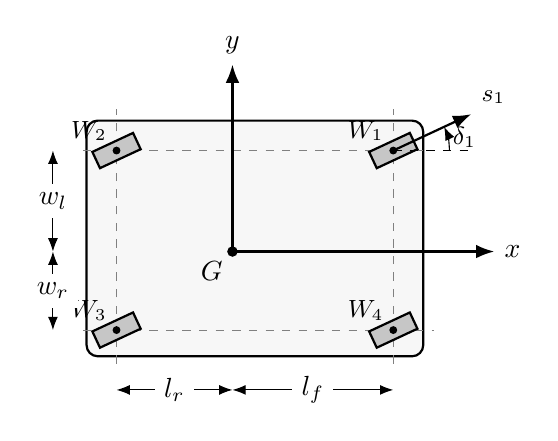
\begin{tikzpicture}[>=Latex,scale=0.95]
    % 以下数值仅用于示意，不代表底盘实测尺寸
    \def\lf{2.15}
    \def\lr{1.55}
    \def\wl{1.35}
    \def\wr{1.05}

    \draw[thick,rounded corners=4pt,fill=gray!6]
        (-1.95,-1.4) rectangle (2.55,1.75);

    \draw[dashed,gray] (-\lr,-1.5)--(-\lr,1.9);
    \draw[dashed,gray] (\lf,-1.5)--(\lf,1.9);
    \draw[dashed,gray] (-2,\wl)--(2.7,\wl);
    \draw[dashed,gray] (-2,-\wr)--(2.7,-\wr);

    \fill (0,0) circle (2pt);
    \node[below left] at (0,0) {$G$};

    \draw[->,thick] (0,0)--(3.5,0)
        node[right] {$x$};
    \draw[->,thick] (0,0)--(0,2.5)
        node[above] {$y$};

    \foreach \xx/\yy/\id in {
        2.15/1.35/1,
        -1.55/1.35/2,
        -1.55/-1.05/3,
        2.15/-1.05/4
    }{
        \begin{scope}[shift={(\xx,\yy)},rotate=25]
            \draw[thick,fill=gray!45]
                (-0.3,-0.12) rectangle (0.3,0.12);
        \end{scope}
        \fill (\xx,\yy) circle (1.5pt);
        \node[above left,font=\small]
            at (\xx,\yy) {$W_{\id}$};
    }

    \draw[dashed] (\lf,\wl)--++(1.1,0);
    \draw[->,thick]
        (\lf,\wl)--++(25:1.15)
        node[above right,font=\small] {$s_1$};

    \draw[->]
        (\lf+0.75,\wl)
        arc[start angle=0,end angle=25,radius=0.75];
    \node[font=\small]
        at (\lf+0.95,\wl+0.18) {$\delta_1$};

    \draw[<->] (0,-1.85)--(\lf,-1.85)
        node[midway,fill=white] {$l_f$};
    \draw[<->] (-\lr,-1.85)--(0,-1.85)
        node[midway,fill=white] {$l_r$};

    \draw[<->] (-2.4,0)--(-2.4,\wl)
        node[midway,fill=white] {$w_l$};
    \draw[<->] (-2.4,-\wr)--(-2.4,0)
        node[midway,fill=white] {$w_r$};
\end{tikzpicture}
\caption{四轮独立转向驱动底盘运动学几何示意图（非比例绘制）}
\label{fig:kc-layout}
\end{figure}

\section{建模假设与单轮运动关系}

\subsection{建模假设}

为建立底盘平面运动学模型，作如下假设：

\begin{enumerate}
    \item 底盘视为平面刚体，忽略车架变形及俯仰、侧倾运动；
    \item 四个车轮与地面保持接触，满足纯滚动和无侧向滑移条件；
    \item 车轮安装位置及有效滚动半径在建模过程中保持不变；
    \item 将转向轴视为通过车轮接地点的竖直投影位置，
          忽略转向轴偏置及转向运动引起的附加速度。
\end{enumerate}

上述假设用于描述理想运动关系。实际运行中，轮胎变形、地面不平、车轮滑移及执行器跟踪误差可能使车轮运动偏离理想模型，其影响需要通过反馈分析和实车试验进行评估。

\subsection{单轮滚动速度}

在纯滚动条件下，第$i$个车轮的有符号滚动线速度为
\begin{equation}
    s_i=r_i\omega_i.
    \label{eq:kc-rolling-speed}
\end{equation}

若驱动器反馈的车轮输出端转速$n_i$以$\mathrm{r/min}$为单位，则
\begin{equation}
    \omega_i=\frac{2\pi}{60}n_i.
    \label{eq:kc-rpm-conversion}
\end{equation}
若反馈来自减速机构输入端，则应先根据传动比换算为车轮输出端转速。

定义车轮滚动方向和侧向的单位向量分别为
\begin{equation}
    \boldsymbol{t}_i
    =
    \begin{bmatrix}
        \cos\delta_i\\
        \sin\delta_i
    \end{bmatrix},
    \qquad
    \boldsymbol{n}_i
    =
    \begin{bmatrix}
        -\sin\delta_i\\
        \cos\delta_i
    \end{bmatrix}.
\end{equation}

第$i$个车轮所在位置的平面速度以车体坐标系表示为$\boldsymbol{u}_i$。在无侧向滑移条件下，
\begin{equation}
    \boldsymbol{n}_i^{T}\boldsymbol{u}_i=0,
    \qquad
    \boldsymbol{t}_i^{T}\boldsymbol{u}_i=s_i.
\end{equation}

因此，
\begin{equation}
    \boldsymbol{u}_i
    =
    \begin{bmatrix}
        u_{ix}\\
        u_{iy}
    \end{bmatrix}
    =
    \begin{bmatrix}
        r_i\omega_i\cos\delta_i\\
        r_i\omega_i\sin\delta_i
    \end{bmatrix}.
    \label{eq:kc-wheel-components}
\end{equation}

该式将单轮滚动速度转换为车体坐标系中的两个速度分量，为正、逆运动学建模提供基础。

\section{底盘逆运动学模型}

\subsection{车体速度与各轮速度的关系}

逆运动学的目标是根据期望车体速度，计算各车轮所需的转向角和驱动轮速。对于刚体底盘，第$i$个车轮所在位置的速度由参考点$G$的平移速度与车体旋转引起的速度叠加得到：
\begin{equation}
    \begin{bmatrix}
        u_{ix}\\
        u_{iy}\\
        0
    \end{bmatrix}
    =
    \begin{bmatrix}
        v_x\\
        v_y\\
        0
    \end{bmatrix}
    +
    \begin{bmatrix}
        0\\
        0\\
        \omega_z
    \end{bmatrix}
    \times
    \begin{bmatrix}
        x_i\\
        y_i\\
        0
    \end{bmatrix}.
\end{equation}

展开后得到
\begin{equation}
\begin{aligned}
    u_{ix}&=v_x-y_i\omega_z,\\
    u_{iy}&=v_y+x_i\omega_z.
\end{aligned}
\label{eq:kc-rigid-velocity}
\end{equation}

其中，$-y_i\omega_z$和$x_i\omega_z$分别为车体旋转在该轮位置产生的纵向和横向速度分量。

对于式\eqref{eq:kc-wheel-coordinates}所示的几何布局，四轮速度分别为
\begin{equation}
\begin{aligned}
    \boldsymbol{u}_1
    &=
    \begin{bmatrix}
        v_x-w_l\omega_z\\
        v_y+l_f\omega_z
    \end{bmatrix},&
    \boldsymbol{u}_2
    &=
    \begin{bmatrix}
        v_x-w_l\omega_z\\
        v_y-l_r\omega_z
    \end{bmatrix},\\[2mm]
    \boldsymbol{u}_3
    &=
    \begin{bmatrix}
        v_x+w_r\omega_z\\
        v_y-l_r\omega_z
    \end{bmatrix},&
    \boldsymbol{u}_4
    &=
    \begin{bmatrix}
        v_x+w_r\omega_z\\
        v_y+l_f\omega_z
    \end{bmatrix}.
\end{aligned}
\label{eq:kc-four-wheel-velocity}
\end{equation}

由此可见，各轮目标速度同时受到车体平移、车体旋转及车轮安装位置的影响，不能在一般复合运动中直接将四个驱动轮设置为相同速度。

\subsection{目标转向角与驱动轮速计算}

设期望车体速度为
\begin{equation}
    \boldsymbol{\xi}^{d}
    =
    \begin{bmatrix}
        v_x^{d} & v_y^{d} & \omega_z^{d}
    \end{bmatrix}^{T},
\end{equation}
则第$i$个车轮的期望速度分量为
\begin{equation}
\begin{aligned}
    u_{ix}^{d}&=v_x^{d}-y_i\omega_z^{d},\\
    u_{iy}^{d}&=v_y^{d}+x_i\omega_z^{d}.
\end{aligned}
\end{equation}

定义目标速度幅值
\begin{equation}
    \rho_i
    =
    \sqrt{
        (u_{ix}^{d})^2+(u_{iy}^{d})^2
    }.
    \label{eq:kc-speed-magnitude}
\end{equation}

当$\rho_i$不为零时，原始目标方向为
\begin{equation}
    \theta_i
    =
    \operatorname{atan2}
    \left(
        u_{iy}^{d},u_{ix}^{d}
    \right).
    \label{eq:kc-raw-angle}
\end{equation}

若该方向满足转向范围要求，则一组可行解为
\begin{equation}
    \delta_i^{d}=\theta_i,
    \qquad
    \omega_i^{d}=\frac{\rho_i}{r_i}.
    \label{eq:kc-basic-inverse}
\end{equation}

当$\rho_i$接近零时，目标滚动方向对数值扰动较为敏感，且零速度本身不要求唯一轮向。因此，设置速度阈值$\varepsilon_v$，当$\rho_i\leq\varepsilon_v$时，将该轮驱动速度设为零，并保持上一有效转向目标，避免静止附近出现无意义的轮向变化。若系统主动进入停车转向状态，则可单独指定其调整目标。

\subsection{有限转角下的等效轮向选择}

由于车轮能够正反向驱动，同一平面速度向量可以由相差$\pi$的轮向与相反的驱动速度共同实现：
\begin{equation}
    s_i
    \begin{bmatrix}
        \cos\delta_i\\
        \sin\delta_i
    \end{bmatrix}
    =
    -s_i
    \begin{bmatrix}
        \cos(\delta_i+\pi)\\
        \sin(\delta_i+\pi)
    \end{bmatrix}.
    \label{eq:kc-equivalent-direction}
\end{equation}

定义第$i$个转向机构的软件允许范围为
\begin{equation}
    \delta_i\in
    [\delta_{i,\min},\delta_{i,\max}].
    \label{eq:kc-steering-limit}
\end{equation}

本平台转向机构受到线缆缠绕限制，研究中按$[-90^\circ,90^\circ]$的受限转向行程建模。实际控制时还需通过安全检查确定限位余量，保证软件目标不超过机械允许范围。

根据原始目标方向$\theta_i$，构造允许范围内的候选轮向：
\begin{equation}
    \mathcal{C}_i
    =
    \left\{
        \theta_i+k\pi
        \;\middle|\;
        k\in\mathbb{Z},\;
        \delta_{i,\min}
        \leq\theta_i+k\pi
        \leq\delta_{i,\max}
    \right\}.
    \label{eq:kc-candidate-set}
\end{equation}

对于候选角$\theta_i+k\pi$，相应的驱动角速度为
\begin{equation}
    \omega_i^{(k)}
    =
    (-1)^k\frac{\rho_i}{r_i}.
    \label{eq:kc-candidate-speed}
\end{equation}

当存在多个可行候选时，可依据当前实际转角$\delta_i^{a}$，选择允许行程内转角变化较小的解：
\begin{equation}
    k_i^{*}
    =
    \underset{
        k:\,\theta_i+k\pi\in\mathcal{C}_i
    }{\operatorname{arg\,min}}
    \left|
        \theta_i+k\pi-\delta_i^{a}
    \right|.
    \label{eq:kc-angle-selection}
\end{equation}

最终目标为
\begin{equation}
    \delta_i^{d}=\theta_i+k_i^{*}\pi,
    \qquad
    \omega_i^{d}
    =
    (-1)^{k_i^{*}}\frac{\rho_i}{r_i}.
    \label{eq:kc-selected-inverse}
\end{equation}

对于具有线缆及行程限制的转向机构，角度差应按实际允许行程计算，不能仅通过周期角度归一化认定存在一条可行的最短旋转路径。候选解代价接近时，可优先保持原有等效分支，并设置切换滞回，减少反馈噪声引起的反复切换。

若$\mathcal{C}_i$为空，则当前车体速度无法通过该轮的允许转向范围实现，应拒绝直接执行，并请求调整车体速度。不得仅将目标转角截断到限位值后继续使用原轮速，否则会破坏期望运动关系。

\section{底盘正运动学模型}

\subsection{四轮联合运动方程}

正运动学根据各轮实际转角和驱动轮速，估计车体速度。设反馈值分别为$\delta_i^{a}$和$\omega_i^{a}$，则由式\eqref{eq:kc-wheel-components}得到
\begin{equation}
    \boldsymbol{b}
    =
    \begin{bmatrix}
        r_1\omega_1^{a}\cos\delta_1^{a}\\
        r_1\omega_1^{a}\sin\delta_1^{a}\\
        r_2\omega_2^{a}\cos\delta_2^{a}\\
        r_2\omega_2^{a}\sin\delta_2^{a}\\
        r_3\omega_3^{a}\cos\delta_3^{a}\\
        r_3\omega_3^{a}\sin\delta_3^{a}\\
        r_4\omega_4^{a}\cos\delta_4^{a}\\
        r_4\omega_4^{a}\sin\delta_4^{a}
    \end{bmatrix}.
    \label{eq:kc-feedback-vector}
\end{equation}

将四轮刚体速度关系联合，可写为
\begin{equation}
    \boldsymbol{b}
    =
    \boldsymbol{A}\boldsymbol{\xi},
    \label{eq:kc-forward-system}
\end{equation}
其中
\begin{equation}
    \boldsymbol{A}
    =
    \begin{bmatrix}
        1&0&-y_1\\
        0&1&x_1\\
        1&0&-y_2\\
        0&1&x_2\\
        1&0&-y_3\\
        0&1&x_3\\
        1&0&-y_4\\
        0&1&x_4
    \end{bmatrix}.
    \label{eq:kc-geometry-matrix}
\end{equation}

对于式\eqref{eq:kc-wheel-coordinates}所示布局，
\begin{equation}
    \boldsymbol{A}
    =
    \begin{bmatrix}
        1&0&-w_l\\
        0&1&l_f\\
        1&0&-w_l\\
        0&1&-l_r\\
        1&0&w_r\\
        0&1&-l_r\\
        1&0&w_r\\
        0&1&l_f
    \end{bmatrix}.
    \label{eq:kc-asymmetric-matrix}
\end{equation}

上述模型使用实际几何关系，不需要假设底盘前后及左右完全对称。

\subsection{基于最小二乘的车体速度估计}

四轮反馈提供八个速度分量，而车体速度包含三个未知量，因此联合运动方程为超定方程组。实际反馈受到轮径误差、转角误差、车轮滑移及数据不同步等因素影响，各方程通常不能被同时精确满足。

采用最小二乘方法估计车体速度：
\begin{equation}
    \hat{\boldsymbol{\xi}}
    =
    \underset{\boldsymbol{\xi}}
    {\operatorname{arg\,min}}
    \left\|
        \boldsymbol{A}\boldsymbol{\xi}
        -
        \boldsymbol{b}
    \right\|_2^2.
    \label{eq:kc-ls-objective}
\end{equation}

当$\boldsymbol{A}$列满秩时，
\begin{equation}
    \hat{\boldsymbol{\xi}}
    =
    \left(
        \boldsymbol{A}^{T}\boldsymbol{A}
    \right)^{-1}
    \boldsymbol{A}^{T}\boldsymbol{b}.
    \label{eq:kc-ls-solution}
\end{equation}

软件实现可采用QR分解或奇异值分解求解，避免直接进行矩阵求逆。用于构造$\boldsymbol{b}$的转角和轮速应尽量对应同一时刻。

定义
\begin{equation}
    S_x=\sum_{i=1}^{4}x_i,
    \qquad
    S_y=\sum_{i=1}^{4}y_i,
    \qquad
    S_r=\sum_{i=1}^{4}(x_i^2+y_i^2),
\end{equation}
则正规方程可展开为
\begin{equation}
    \begin{bmatrix}
        4&0&-S_y\\
        0&4&S_x\\
        -S_y&S_x&S_r
    \end{bmatrix}
    \begin{bmatrix}
        \hat v_x\\
        \hat v_y\\
        \hat\omega_z
    \end{bmatrix}
    =
    \begin{bmatrix}
        \displaystyle\sum_{i=1}^{4}u_{ix}\\[2mm]
        \displaystyle\sum_{i=1}^{4}u_{iy}\\[2mm]
        \displaystyle\sum_{i=1}^{4}
        (-y_i u_{ix}+x_i u_{iy})
    \end{bmatrix}.
    \label{eq:kc-normal-equation}
\end{equation}

由此可见，只有当参考点满足$S_x=S_y=0$时，车体平移速度才能直接由各轮速度分量的算术平均得到。对于一般非对称布局，应保留完整几何矩阵进行求解。

定义运动学残差
\begin{equation}
    \boldsymbol{e}
    =
    \boldsymbol{b}
    -
    \boldsymbol{A}\hat{\boldsymbol{\xi}},
    \label{eq:kc-residual}
\end{equation}
用于描述四轮反馈与所估计刚体运动之间的不一致程度。较大的残差可能与滑移、标定误差或反馈不同步有关，但不能仅凭残差确定故障来源。多轮同时发生相近程度的纵向滑移时，残差仍可能较小，因此其不能替代外部定位观测。

\subsection{轮式里程计计算}

正运动学估计的平移速度在车体坐标系中表达，转换至世界坐标系后有
\begin{equation}
    \begin{bmatrix}
        \dot X\\
        \dot Y\\
        \dot\psi
    \end{bmatrix}
    =
    \begin{bmatrix}
        \cos\psi&-\sin\psi&0\\
        \sin\psi&\cos\psi&0\\
        0&0&1
    \end{bmatrix}
    \begin{bmatrix}
        \hat v_x\\
        \hat v_y\\
        \hat\omega_z
    \end{bmatrix}.
    \label{eq:kc-world-velocity}
\end{equation}

设相邻两次更新的时间间隔为$\Delta t$，采用前向欧拉积分可得
\begin{equation}
\begin{aligned}
    X_{k+1}
    &=
    X_k+
    \left(
        \hat v_{x,k}\cos\psi_k
        -
        \hat v_{y,k}\sin\psi_k
    \right)\Delta t,\\
    Y_{k+1}
    &=
    Y_k+
    \left(
        \hat v_{x,k}\sin\psi_k
        +
        \hat v_{y,k}\cos\psi_k
    \right)\Delta t,\\
    \psi_{k+1}
    &=
    \psi_k+\hat\omega_{z,k}\Delta t.
\end{aligned}
\label{eq:kc-odometry}
\end{equation}

时间间隔应根据有效反馈时间戳确定。轮式里程计描述相对于初始状态的运动，其误差会随积分累积，后续可结合IMU、激光雷达或视觉观测进行修正。在停车调整轮向及明显滑移阶段，纯滚动假设可能受到破坏，应对相应里程计结果降低置信度。

\section{轮级指令生成与执行}

\subsection{控制系统总体结构}

底盘运动控制的目标方案采用Jetson与STM32分工的结构。Jetson接收有效车体速度请求，完成指令平滑、逆运动学解算、等效轮向选择及转向与驱动协调，生成四轮转向位置和驱动轮速目标；拟开发的STM32控制板完成指令检查、电机协议转换、CAN报文调度及状态采集，并独立执行通信超时和故障保护。在STM32硬件完成前，上述电机协议转换和CAN通信由Jetson侧驱动临时完成。

电机内部驱动器承担其支持的位置、速度及电流闭环，Jetson侧协调模块依据实际转角和轮速判断运动执行状态，不以目标已发送作为执行完成的依据。控制系统主要信号关系如图\ref{fig:kc-control-structure}所示。

\begin{figure}[htbp]
\centering
\begin{tikzpicture}[
    >=Latex,
    node distance=10mm,
    block/.style={
        draw,
        rounded corners,
        align=center,
        font=\small,
        text width=64mm,
        minimum height=11mm
    },
    flow/.style={->,thick}
]
    \node[block] (input)
        {有效车体速度请求};

    \node[block,below=of input] (jet)
        {Jetson\\指令平滑、逆运动学与运动协调};

    \node[block,below=of jet] (stm)
        {STM32\\指令检查、通信调度与安全保护};

    \node[block,below=of stm] (motor)
        {电机驱动器与执行器\\转向位置及驱动速度控制};

    \draw[flow] (input)--(jet);

    \draw[flow] (jet)--node[right,font=\scriptsize]
        {四轮目标}(stm);

    \draw[flow] (stm)--node[right,font=\scriptsize]
        {电机控制报文}(motor);

    \draw[flow]
        (motor.west)--++(-12mm,0)
        |-node[pos=0.25,left,font=\scriptsize]
        {电机反馈}(stm.west);

    \draw[flow]
        (stm.east)--++(16mm,0)
        |-node[pos=0.25,right,align=left,font=\scriptsize]
        {转角、轮速\\及运行状态}(jet.east);
\end{tikzpicture}
\caption{底盘运动控制及反馈结构}
\label{fig:kc-control-structure}
\end{figure}

为保持控制逻辑一致，底盘几何参数、车轮编号、转角零位、驱动方向和单位换算应统一配置。规划中的STM32不重复执行车体逆运动学，也不在正常执行过程中独立切换等效轮向分支；但应对接收到的转角、轮速、序号和时效进行独立校验，拒绝越界或过期目标。

\subsection{转向与行走的执行协调}

逆运动学给出期望轮向与轮速，执行模块依据实际转角和轮速判断运动状态。小幅轮向调整时限制行走速度；大幅调整或等效轮向分支切换时，采用减速停车、零速转向和恢复行走的顺序。停车与转向完成均依据反馈确认，不以固定延时代替。

上述内容仅说明轮级指令的基本执行方式。有限转向角对速度规划的影响将在第\ref{chap:steering-planning}章讨论。

\subsection{轮速限幅与安全处理}

轮速目标超过执行器允许范围时，按统一比例缩放四轮速度，保持轮间目标比例。对转向位置、转向速度、驱动轮速及指令时效分别进行检查；转角越界时不能直接截断角度并继续执行原驱动速度。实际参数和停车阈值根据标定及试验确定。

目标系统中，通信超时、反馈失效及执行器故障由STM32独立保护逻辑处理，并将状态上传Jetson。STM32尚未接入时，由Jetson侧控制器超时和驱动器通信保护承担过渡阶段的失联停车功能。无论采用何种硬件结构，异常解除后均需重新确认使能条件，不自动恢复过期运动请求。

\section{本章小结}

本章针对非对称四轮独立转向驱动底盘，建立了坐标系、车轮几何描述及单轮滚动模型，推导了由车体速度生成四轮转向角与驱动轮速的逆运动学关系，并给出了有限转角下基于驱动反转的等效轮向选择方法。

在此基础上，建立四轮联合正运动学方程，采用最小二乘方法估计车体速度，并给出轮式里程计的计算过程。本章进一步明确轮级目标生成与执行接口，为后续有限转向角规划方法提供运动学基础。


\chapter{多层棚架环境感知与三维语义建图}
\label{chap:perception-mapping}

温室多层棚架存在结构重复、上下层叠置及局部遮挡等特点。仅依靠二维占据栅格无法表达棚架的对象身份与层级关系。为此，本章以RGB-D观测为主要输入，利用定位结果将多帧观测统一至地图坐标系，在常规几何地图之外构建包含棚架对象、层面及其几何属性的语义地图。相关识别、融合和关联算法仍属于待实现和验证的研究内容。

\section{环境感知与定位建图方案}

机器人采用D435i相机获取彩色图像、深度图与内参，使用激光雷达获取二维扫描。底盘里程计提供连续运动估计，RTAB-Map结合RGB-D观测与里程计先验进行定位和全局地图维护，Nvblox在外部位姿输入下进行局部三维重建。传感器安装变换通过ROS~2坐标变换系统统一管理。激光及IMU是否参与融合以实际联调结果为准。

\placeholderfigure{5cm}{系统流程图（待补充）：RGB-D／里程计／RTAB-Map／Nvblox／棚架语义地图}{环境感知与语义建图总体流程}{fig:sem-framework}

\subsection{定位与坐标关系}

设地图坐标系、里程计坐标系、车体坐标系与相机光学坐标系分别为$\{M\}$、$\{O\}$、$\{B\}$和$\{C\}$。若$^{A}\boldsymbol{T}_{B}$表示从坐标系$\{B\}$至$\{A\}$的齐次变换，则相机观测点转换到全局地图坐标系的过程为
\begin{equation}
{}^{M}\tilde{\boldsymbol p}
={}^{M}\boldsymbol T_O\,{}^{O}\boldsymbol T_B\,
 {}^{B}\boldsymbol T_C\,{}^{C}\tilde{\boldsymbol p}.
\label{eq:sem-global-transform}
\end{equation}
其中$^{O}\boldsymbol T_B$由连续里程计估计，$^{M}\boldsymbol T_O$由全局定位维护，$^{B}\boldsymbol T_C$由相机外参标定确定。进行多帧关联时必须使用与图像时间戳一致的变换；在定位回环修正后，应维护对象地图的坐标一致性。

\subsection{Nvblox三维几何地图}

Nvblox接收深度观测、相机内参与位姿，在体素网格中融合截断有符号距离场（TSDF），用于表示观测表面附近的几何结构。由TSDF可生成表面网格（Mesh）和用于空间距离查询的欧氏有符号距离场（ESDF）。其中，TSDF主要服务于多帧几何重建，ESDF可为局部障碍距离计算及轨迹安全性评价提供输入。

\begin{equation}
D_{\mathrm{TSDF}}(\boldsymbol p)
=\operatorname{clip}\!\left(d_s(\boldsymbol p),-\mu,\mu\right),
\label{eq:sem-tsdf}
\end{equation}
式中$d_s$表示带符号的表面距离，$\mu$为截断距离。上式为TSDF的概念性定义；实际实现需结合相机射线、距离符号约定和体素加权融合。Nvblox不自动给出棚架ID或层级关系，本研究将三维几何重建与独立的语义对象地图分开维护。

% 待补充：Nvblox融合参数、局部Mesh及ESDF实际截图。
\placeholderfigure{4.5cm}{Nvblox Mesh／ESDF 可视化结果（待补充）}{局部三维环境重建与距离场示例}{fig:sem-nvblox}

\section{棚架目标识别与空间几何提取}

\subsection{RGB-D实例分割与点云恢复}

拟采用棚架或层面实例分割网络获得各目标像素掩膜。对于深度已经对齐到彩色相机的有效像素$(u,v)$，由针孔相机模型恢复三维点：
\begin{equation}
{}^{C}\boldsymbol p(u,v)
=\begin{bmatrix}
(u-c_x)Z(u,v)/f_x\\
(v-c_y)Z(u,v)/f_y\\
Z(u,v)
\end{bmatrix},
\label{eq:sem-backprojection}
\end{equation}
其中$f_x,f_y,c_x,c_y$为相机内参，$Z$为有效深度。按实例掩膜筛选点集，去除无效点和明显离群点，再由式\eqref{eq:sem-global-transform}统一到地图坐标系。棚架的训练数据、网络结构及检测性能将在完成实验后补充。

\subsection{层面几何与朝向估计}

棚架层面可用中心位置、高度、平面主方向与边界尺寸近似描述。设某层面的有效二维点集为$\{\boldsymbol p_j\}_{j=1}^{N}$，先计算点集中心$\bar{\boldsymbol p}$和协方差矩阵：
\begin{equation}
\bar{\boldsymbol p}=\frac{1}{N}\sum_{j=1}^{N}\boldsymbol p_j,
\qquad
\boldsymbol\Sigma=\frac{1}{N}\sum_{j=1}^{N}
(\boldsymbol p_j-\bar{\boldsymbol p})
(\boldsymbol p_j-\bar{\boldsymbol p})^T.
\label{eq:sem-pca}
\end{equation}
对$\boldsymbol\Sigma$进行特征值分解，以最大特征值对应的特征向量估计层面主方向，并沿主轴及其正交轴统计点集分布，得到可见区域的边界估计。层面高度由对应三维点的高度分布确定，多个层面再依据高度差及水平投影关系进行层级组织。

由于局部遮挡会使点集不完整，单帧提取结果只能代表已观测区域，不能直接认定为棚架真实尺寸。对于层面倾斜、相邻棚架紧密排列等情况，可引入平面拟合或多视角补全，并在后续实验中比较方法稳定性。

\placeholderfigure{5cm}{RGB图像／实例掩膜／层面点云／拟合边界（待补充）}{棚架识别及三维几何特征提取}{fig:sem-geometry}

\section{多帧关联与结构化语义地图}

\subsection{对象关联与地图更新}

不同视角下，同一棚架可能被多次观测，需要通过空间位置、层面高度、主方向和边界重叠关系建立观测与地图对象的对应。记新观测对象为$z_j$，已有地图对象为$m_i$，可构造关联代价：
\begin{equation}
C_{ij}=\lambda_p\frac{\|\boldsymbol c(z_j)-\boldsymbol c(m_i)\|_2}{d_0}
+\lambda_h\frac{|h(z_j)-h(m_i)|}{h_0}
+\lambda_\theta\frac{\Delta\theta(z_j,m_i)}{\theta_0},
\label{eq:sem-assoc}
\end{equation}
其中$\boldsymbol c$为层面中心，$h$为高度，$\Delta\theta$为考虑主轴方向等价性的角度差；$d_0,h_0,\theta_0$用于归一化。经关联门控后，可采用一对一匹配方法建立观测对应关系；代价形式及权重属于待验证方案。

完成匹配后，根据观测置信度更新对象几何参数；未匹配观测经过多帧确认后建立新对象，短时未观测对象保留历史状态。通过这种方式避免因遮挡或视角变化导致每帧重新编号。

\subsection{语义地图的数据表达}

语义地图采用“棚架--层面”的层级组织形式。每个棚架记录唯一ID、全局参考位姿及所属层面集合；每个层面记录层面ID、相对高度、中心、主方向、边界、观测时间及置信信息。可用如下结构表示：
\begin{equation}
\mathcal M_{\mathrm{sem}}
=\big\{R_j,\; R_j=(\mathrm{ID}_j,\boldsymbol T_j,
 \{L_{j,k}\}_{k=1}^{K_j})\big\},
\label{eq:sem-map}
\end{equation}
其中$L_{j,k}$表示第$j$个棚架的第$k$层结构及其几何属性。棚架行列关系和具体编号规则将在多视角关联方案确定后完善。几何地图与语义地图相互关联，但不将语义对象直接等同于障碍物占据体素。

% 待补充：语义地图消息结构与ROS 2发布接口。
\placeholderfigure{5cm}{棚架ID、层级编号、三维边界及机器人位置（待补充）}{多层棚架结构化语义地图示例}{fig:sem-rack-map}

\section{本章小结}

本章给出了基于RGB-D、RTAB-Map和Nvblox的环境感知基础架构，并提出面向多层棚架的实例识别、三维几何提取、跨帧关联及层级语义地图表达方案。算法实现与性能评价将在实验阶段完成。


\chapter{有限转向角约束下的四轮运动规划方法}
\label{chap:steering-planning}

本章在第\ref{chap:kinematics-control}章四轮运动学模型的基础上，分析有限转向角引起的轮向切换问题，介绍将转向约束引入ROS~2 Nav2局部规划器的基本思路。具体规划算法尚待实现，以下内容主要给出约束模型及后续设计方向。

\section{有限转向角下的速度空间分析}

根据第\ref{chap:kinematics-control}章的逆运动学关系，第$i$个车轮的平面速度为
\begin{equation}
\boldsymbol{u}_i=
\begin{bmatrix}
 v_x-y_i\omega_z\\
 v_y+x_i\omega_z
\end{bmatrix}.
\label{eq:pl-wheel-velocity}
\end{equation}
当车轮转角限制为$[-\pi/2,\pi/2]$时，可通过驱动轮正反转实现等效的速度方向。但当车轮速度方向跨过转向角边界时，目标转角可能出现跳变，从而需要切换等效轮向分支。

令轮速纵向分量为零，得到速度空间中的候选切换边界：
\begin{equation}
H_i:\quad v_x-y_i\omega_z=0.
\label{eq:pl-switch-boundary}
\end{equation}
若左侧车轮的横向位置为$w_l$，右侧车轮为$-w_r$，则有
\begin{equation}
\begin{aligned}
H_l:&\quad v_x-w_l\omega_z=0,\\
H_r:&\quad v_x+w_r\omega_z=0.
\end{aligned}
\label{eq:pl-switch-planes}
\end{equation}
上述边界仅表征等效轮向可能发生切换的位置，是否需要实际调整车轮还取决于当前轮向和具体速度变化。文献\cite{liu2025constrained}已对有限转角速度空间中的不连续平面进行了研究，本研究将其作为后续规划器设计的理论基础。

% 待补充：速度空间切换边界示意图。
\placeholderfigure{5cm}{速度空间切换边界图（待补充）}{有限转向角下的速度空间分区}{fig:pl-discontinuity}

\section{局部规划器设计思路}

机器人导航采用ROS~2 Nav2框架。局部规划器根据路径、障碍物信息和当前运动状态生成车体速度指令，随后由四轮逆运动学模块计算各轮转向角和驱动轮速。

对于候选车体速度$\boldsymbol\xi^d$，首先利用第\ref{chap:kinematics-control}章的等效轮向求解方法检查是否存在满足转角范围的轮级目标；然后结合当前轮向判断候选指令是否可能引起分支切换。在此基础上，可研究将转向分支切换惩罚加入局部规划器的评价过程。

候选轨迹的评价可写为一般形式：
\begin{equation}
J(\tau)=J_{\mathrm{nav}}(\tau)+\lambda_f J_{\mathrm{flip}}(\tau),
\label{eq:pl-cost}
\end{equation}
其中$J_{\mathrm{nav}}$表示规划器原有的路径跟踪与避障等代价，$J_{\mathrm{flip}}$表示轮向切换相关代价，$\lambda_f$为权重。该式是规划设计的初步表达，并非已经完成验证的改进算法。实际采用DWB、MPPI或其他局部控制器，以及评价函数的具体形式，将在实现阶段确定。

% 待补充：所选Nav2局部规划器及其接口。
% 待补充：转向约束评价函数和实际实现细节。

\section{本章小结}

本章分析了有限转向角下的速度空间切换边界，并给出将轮向切换约束引入Nav2局部规划器的初步思路。后续工作将根据实际算法实现情况补充。


\begin{thebibliography}{9}
\bibitem{liu2025constrained}
Liu S, Had\v{z}i\'{c} I, Gupta A, Arab A.
Motion Planning and Control of an Overactuated 4-Wheel Drive with Constrained Independent Steering[EB/OL].
arXiv:2510.19054, 2025.
\end{thebibliography}

\end{document}
